\documentclass{article}

\usepackage{amsmath, parskip, tikz}
\usetikzlibrary{automata}
\usetikzlibrary{positioning}
\usetikzlibrary{arrows}
\usepackage[margin=1.25in]{geometry}
\usepackage[shortlabels]{enumitem}

\newcommand\blanksymbol\textvisiblespace

\renewcommand{\thesection}{\arabic{section}.}
\renewcommand{\thesubsection}{\alph{section}.}

\tikzset{
    node distance=2.5cm,
    every state/.append style={
        semithick,
        fill=gray!10
    },
    initial/.append style={
        initial text={},
        initial distance=0.5cm
    },
    accepting/.append style={
        double=gray!10,
        double distance=2pt,
        outer sep=1pt
    },
    every edge/.append style={
        draw,
        ->,>=stealth',
        auto,
        semithick
    }
}

\title{Homework 6: Turing Machine Variants}
\author{Will Griffin}

\begin{document}
    \maketitle

    \section{Doubly infinite tapes}

    A Turing machine with a doubly infinite tape is like a TM but with a tape that extends infinitely in both directions. Initially, the head is at the first symbol of the input string, but there are infinitely many blanks to the right.

    Show how, given a TM with a doubly infinite tape, to construct an equivalent standard, single-tape TM. An \textbf{implementation description} in the style of Proof 3.13 is fine, and it's also fine to use any results proved in the book or in class.

    Given a doubly infinite taped TM $D$, an equivalent standard TM $M$ can be constructed with the instruction set

    $M = $ ``On input $w$
    \begin{enumerate}
        \item Shift every symbol to the right by one space. Then, move the head to the left end and write some symbol $c_\text{R}$ where $c_\text{R} \text{ (and future $c_\text{L}$)} \notin \Gamma_D$ to mark the end of the tape. 

        \item Then, shift symbols of the input string $w$ such that there is a $\text{\blanksymbol} $ between every symbol of $w$.

        \item Move the head to the first symbol of $w$.

        \item $M$ will remember which side of the tape it is on in reference to $D$. This is done by switching between $c_\text{R}$ and $c_\text{L}$ as the first symbol. 

        \item Simulate $D$, where left and right moves of the head of $D$ follow the following rules:
            \begin{enumerate}[a.]

                \item While the first symbol is $c_\text{R}$,
                    \begin{enumerate}
                        \item If the next transition is a move to the right, move the head right two spaces.

                        \item If the next transition is a move to the left and the head is not on $w_1$, move the head left two spaces.

                        \item If the next transition is a move to the left and the head is on $w_1$, move the head left once, write $c_\text{L}$, then move the head to the right twice.
                    \end{enumerate}

                \item While the first symbol is $c_\text{L}$,
                    \begin{enumerate}
                        \item If the next transition is a move to the left, move the head right two spaces.

                        \item If the next transition is a move to the right, move the head to the left twice. If the head then reads $c_\text{L}$, write $c_\text{R}$ and then move the head to the right once.
                    \end{enumerate}

            \end{enumerate}
    \end{enumerate}

    \section{Two-stack PDAs}

    Show that any Turing machine $M$ can be converted into an equivalent 2PDA $P$. Use \textbf{formal descriptions} of both $M$ and $P$. Be sure to include in your construction the following:

    \begin{enumerate}[-]
        \item For each state $q$ of $M$, you should create a state $q$ in $P$.
        
        \item If $s$ is the start state of $M$, what should you do?

        \item If $q_\text{accept}$ is the accept state of $M$, what should you do?

        \item If $q_\text{reject}$ is the reject state of $M$, what should you do?

        \item For each transition that looks like this, what should you do?
            \begin{center}
            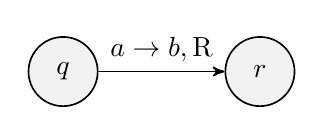
\begin{tikzpicture}
                \node[state] (q) {$q$};
                \node[state, right of=q] (r) {$r$};

                \draw[->] (q) edge node {$a \to b, \text{R}$} (r);
            \end{tikzpicture}
            \end{center}

        \item For each transition that looks like this, what should you do?
            \begin{center}
            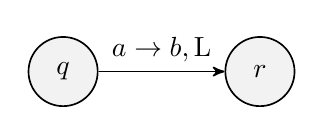
\begin{tikzpicture}
                \node[state] (q) {$q$};
                \node[state, right of=q] (r) {$r$};

                \draw[->] (q) edge node {$a \to b, \text{L}$} (r);
            \end{tikzpicture}
            \end{center}
    \end{enumerate}

    A 2PDA $P$ that is equivalent to a standard Turing machine $M$ can be constructed by the following steps:

    \begin{enumerate}[-]
        \item For each state $q$ in $M$, create state $q$ in $P$.

        \item For the start state $s$ in $M$, create new states $s'_1$, $s'_2$, $s'_3$ in $P$ with the following transitions:
            \begin{center}
            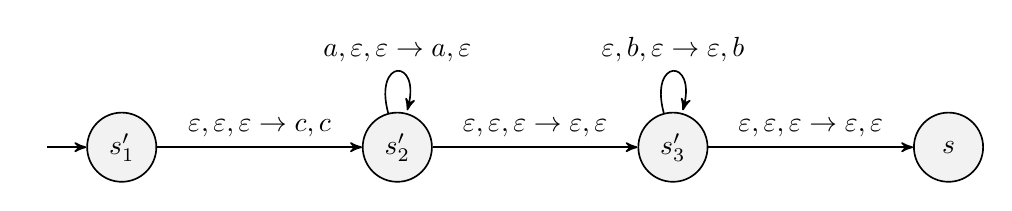
\begin{tikzpicture}
                \node[state, initial, xshift=-1cm] (sp) {$s'_1$};
                \node[state, right of=sp, xshift=1cm] (sp2) {$s'_2$};
                \node[state, right of=sp2, xshift=1cm] (sp3) {$s'_3$};
                \node[state, right of=sp3, xshift=1cm] (s) {$s$};

                \draw (sp) edge node {$\varepsilon, \varepsilon, \varepsilon \to c, c$} (sp2);
                \draw (sp2) edge[loop above] node {$a, \varepsilon, \varepsilon \to a, \varepsilon$} (sp2);
                \draw (sp2) edge node {$\varepsilon, \varepsilon, \varepsilon \to \varepsilon, \varepsilon$} (sp3);
                \draw (sp3) edge[loop above] node {$\varepsilon, b, \varepsilon \to \varepsilon, b$} (sp3);
                \draw (sp3) edge node {$\varepsilon, \varepsilon, \varepsilon \to \varepsilon, \varepsilon$} (s);
            \end{tikzpicture}
            \end{center}

            where $c \notin \Gamma$ and is an end marker, $a, b \in \Sigma$, where transitions including $a$ and $b$ are created for all $a, b \in \Sigma$.

            Essentially, this means that upon reaching $s$, the first stack will contain $c$, a terminal character not in the tape alphabet, and the second stack will contain $w^\text{R}$ where $w$ is the input string and $w_1$ is the top item in the stack.

        \item For the accept state $q_\text{accept}$ in $M$, make $q_\text{accept}$ an accept state in $P$.

        \item For the reject state $q_\text{reject}$ in $M$, ensure state $q_\text{reject}$ exists in $P$.

        \item For each right shift transition in $M$, 
            \begin{center}
            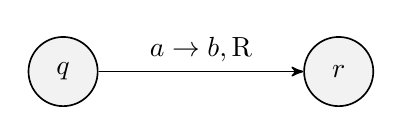
\begin{tikzpicture}
                \node[state, xshift=-1cm] (q) {$q$};
                \node[state, right of=q, xshift=1cm] (r) {$r$};

                \draw (q) edge node {$a \to b, \text{R}$} (r);
            \end{tikzpicture}
            \end{center}

            where $q, r$ are states in $M$, create a transition in $P$ such that

            \begin{center}
            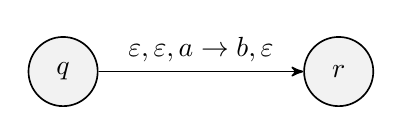
\begin{tikzpicture}
                \node[state, xshift=-1cm] (q) {$q$};
                \node[state, right of=q, xshift=1cm] (r) {$r$};

                \draw (q) edge node {$\varepsilon, \varepsilon, a \to b, \varepsilon$} (r);
            \end{tikzpicture}
            \end{center}

            where $q, r$ are states in $P$ and $a, b \in \Gamma$.

            When $a = $ \blanksymbol, also add the transition

            \begin{center}
            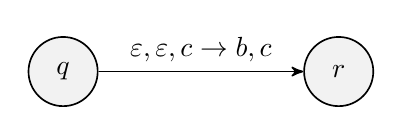
\begin{tikzpicture}
                \node[state, xshift=-1cm] (q) {$q$};
                \node[state, right of=q, xshift=1cm] (r) {$r$};

                \draw (q) edge node {$\varepsilon, \varepsilon, c \to b, c$} (r);
            \end{tikzpicture}
            \end{center}

            where $c \notin \Gamma$ is a stack end marker.

        \item For each left shift transition in $M$, 
            \begin{center}
            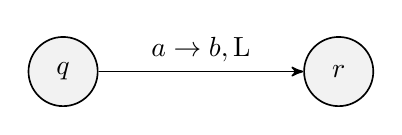
\begin{tikzpicture}
                \node[state, xshift=-1cm] (q) {$q$};
                \node[state, right of=q, xshift=1cm] (r) {$r$};

                \draw (q) edge node {$a \to b, \text{L}$} (r);
            \end{tikzpicture}
            \end{center}

            where $q, r$ are states in $M$, create transitions in $P$ such that

            \begin{center}
            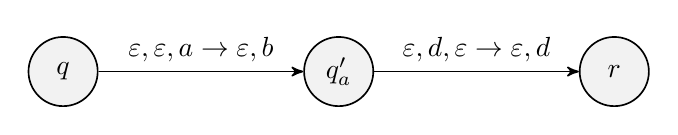
\begin{tikzpicture}
                \node[state, xshift=-1cm] (q) {$q$};
                \node[state, right of=q, xshift=1cm] (qp) {$q'_a$};
                \node[state, right of=qp, xshift=1cm] (r) {$r$};

                \draw (q) edge node {$\varepsilon, \varepsilon, a \to \varepsilon, b$} (qp);
                \draw (qp) edge node {$\varepsilon, d, \varepsilon \to \varepsilon, d$} (r);
            \end{tikzpicture}
            \end{center}

            where $q, r$ are states in $P$ and $a, b, d \in \Gamma$.

            When $a = $ \blanksymbol, also add the transitions

            \begin{center}
            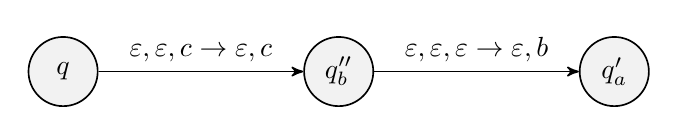
\begin{tikzpicture}
                \node[state, xshift=-1cm] (q) {$q$};
                \node[state, right of=q, xshift=1cm] (qp) {$q''_b$};
                \node[state, right of=qp, xshift=1cm] (r) {$q'_a$};

                \draw (q) edge node {$\varepsilon, \varepsilon, c \to \varepsilon, c$} (qp);
                \draw (qp) edge node {$\varepsilon, \varepsilon, \varepsilon \to \varepsilon, b$} (r);
            \end{tikzpicture}
            \end{center}

            for all $b \in \Gamma$.

            To ensure the "tape does not go past the left end" in $P$, create states $q'_a$ (for all $a \in \Sigma$) and transitions

            \begin{center}
            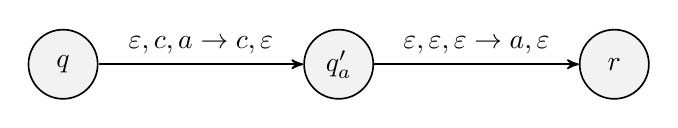
\begin{tikzpicture}
                \node[state, xshift=-1cm] (q) {$q$};
                \node[state, right of=q, xshift=1cm] (qp) {$q'_a$};
                \node[state, right of=qp, xshift=1cm] (r) {$r$};

                \draw (q) edge node {$\varepsilon, c, a \to c, \varepsilon$} (qp);
                \draw (qp) edge node {$\varepsilon, \varepsilon, \varepsilon \to a, \varepsilon$} (r);
            \end{tikzpicture}
            \end{center}

            where $q, r$ are states in $P$, $c \notin \Gamma$ and is an end marker, and $a \in \Sigma$. These transitions are created for all $a \in \Sigma$.

            

    \end{enumerate}

    \section{Brain Fun}

    Give an \textbf{implementation description} of a multitape Turing machine that can interpret any $\mathcal{P}''$ program. The input would be a string $P\texttt{\#}w$ where $P$ is a $\mathcal{P}''$ program and $w$ is an input string, and it should accept iff $P$ accepts $w$.

    A multitape Turing machine $M$ that can interpret $\mathcal{P}''$ programs can be defined by such:

    $M = $ ``On input $u$, where $u = P\texttt{\#}w$

    \begin{enumerate}[1.]
        \item Copy the $w$ part of the input string $u$ to the second tape. This can be done by first moving head 1 right to the \texttt{\#}, then right once more. Then, take whatever symbol $a \in w$ and write it to the second tape, replacing it on the first tape with a \blanksymbol, then moving right head 1 and 2 to the next symbol. Repeat until all symbols of $w$ are read and copied to the second tape.

        \item Move head 1 left until it reaches the \texttt{\#}, and replace it with a \blanksymbol. Then, move head 1 left until it reaches the left end of the tape. Move head 2 left until it reaches the left end of the tape.

        \item Read head 1's symbol, and perform a different action depending on the symbol read:
            \begin{enumerate}[-]
                \item If \texttt{<} is read, move head 2 to the left by one cell if it is not at the left end.

                \item If \texttt{>} is read, move head 2 to the right by one cell.

                \item If \texttt{+} is read, read the symbol under head 2 and write it incremented by one (that is, $a_0$ becomes $a_1$, $a_1$ becomes $a_2$, and so on; $a_{n-1}$ becomes $a_0$).

                \item If \texttt{-} is read, read the symbol under head 2 and write it decremented by one (that is, $a_{n-1}$ becomes $a_{n-2}$, $a_{n-2}$ becomes $a_{n-3}$, and so on; $a_0$ becomes $a_{n-1}$).

                \item If \texttt{[} is read, read the symbol under head 2. If the symbol is $a_0$, move head 1 to the right until it reaches its matching \texttt{]}. Otherwise, if the symbol is anything but $a_0$, continue.

                \item If \texttt{]} is read, move head 1 left until it reaches its corresponding \texttt{[}. Then, move head 1 one more cell to the left, so that the condition check can happen at the start of the loop.

                \item If $\text{\blanksymbol} $ is read, read the symbol under head 2. If the symbol is $a_0$, \textit{reject}, otherwise, \textit{accept}.
            \end{enumerate}

        \item Move head 1 to the right once and go back to step 3.
    \end{enumerate}

    
\end{document}
